最終的にSelf-Attentionメモリー機構は図\ref{fig:self-attention-convlstm}のようにConvLSTMに組み込まれる。

\begin{figure}[H]
\begin{center}
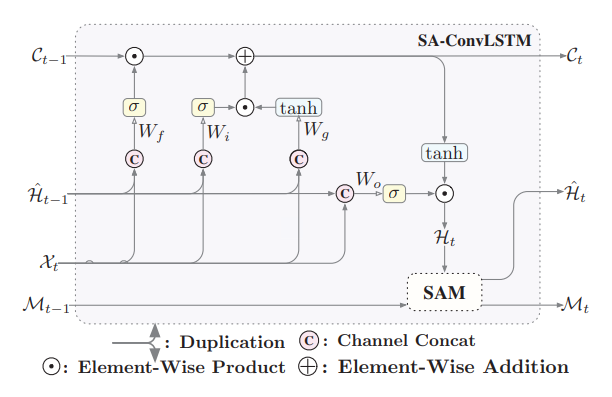
\includegraphics[width=0.9\linewidth]{fig/methodologies/self-attention-convlstm.png}
\captionsetup{width=0.9\linewidth}
\caption{Lin \textit{et al}.[2020] Figure2より引用。Self-Attention ConvLSTMの計算概要図。}
\label{fig:self-attention-convlstm}
\end{center}
\end{figure}

具体的には以下のように計算される。

\begin{align}
\left.
\begin{aligned}
	i_{t} &= \sigma(W_{xi} * X_{t} + W_{hi} * H_{t−1} + W_{ci} \odot \mathcal{C}_{t−1} + b_{i})\\ 
	f_{t} &= \sigma(W_{xf} * X_{t} + W_{hf} * H_{t−1} + W_{cf} \odot \mathcal{C}_{t−1} + b_{f}) \\
	\mathcal{C}_{t} &= f_{t} \odot \mathcal{C}_{t−1} + i_{t} \odot \tanh(W_{xc} * X_{t} + W_{hc} * \mathcal{H}_{t−1} + b_{c}) \\
	o_{t} &= \sigma(W_{xo} * X_{t} + W_{ho} * \mathcal{H}_{t−1} + W_{co} \odot \mathcal{C}_{t} + b_{o}) \\
	\mathcal{H}_{t} &= o_{t} \odot \tanh(\mathcal{C_{t}}) \\
\end{aligned}
\right\} \quad \text{ConvLSTMの処理} \\
\left.
\begin{aligned}
	i'_{t} &= \sigma(W_{m;zi} \ast \boldsymbol{Z} + W_{m;hi} \ast \mathcal{H}_{t} + b_{m;i}) \\
	g'_{t} &= tanh(W_{m;zg} \ast \boldsymbol{Z} + W_{m;hg} \ast \mathcal{H}_{t} + b_{m;g}) \\
	\mathcal{M}_{t} &= (1 - i'_{t}) \circ \mathcal{M}_{t-1} + i'_{t} \circ g'_{t} \\
	o'_{t} &= \sigma(W_{m;zo} \ast \boldsymbol{Z} + W_{m;ho} \ast \mathcal{H}_{t} + b_{m;o}) \\
	\hat{\mathcal{H}}_{t} &= o'_{t} \circ \mathcal{M}_{t}
\end{aligned}
\right\} \quad \text{Self-Attentionメモリー機構の処理}
\end{align}
